\subsubsection{Risultati sperimentali}
In \autoref{fig:obj1_boxplot_utilization} andiamo ad analizzare il comportamento dell'utilizzazione. Per tutti i nodi l'andamento è crescente, come ci aspettavamo, la dispersione è piuttosto simile tra i vari box ad eccezione del server B con tasso di arrivo 1.2$job/s$, in questo caso il box è schiacciato verso 1. Sia il server A che il server B presentano valori di massimo che raggiungono 1, invece per quanto riguarda i valori medi di utilizzazione il valore più alto che troviamo è di 0.97 per il server B quando il tasso di arrivo è 1.2$job/s$, seguito dal caso con tasso di arrivo 1.15$job/s$ ed utilizzazione 0.92 sempre per il server B. Per i valori medi sono gli unici due casi che superano lo 0.9.\\
Da notare anche come le performance del server B influenzino l'andamento del sistema.
\begin{figure*}
    \centering
    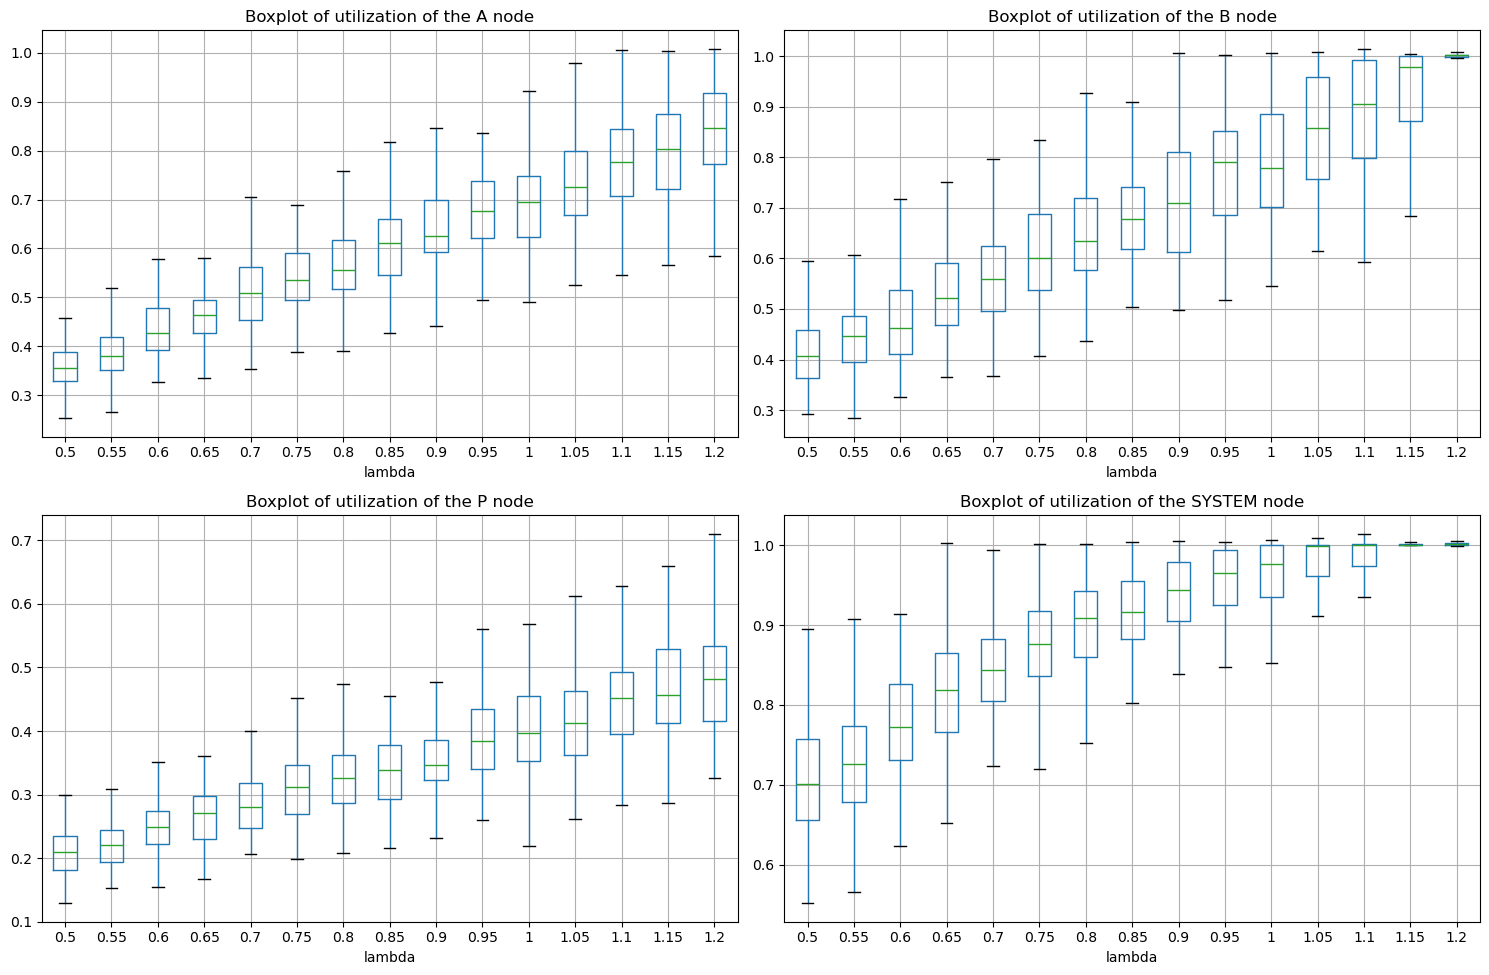
\includegraphics[width=\textwidth]{figs//results/obj1/obj1-box-utilization.png}
    \caption{Distribuzione dell'utilizzazione dei risultati sperimentali dell'obbiettivo 1.}
    \label{fig:obj1_boxplot_utilization}
\end{figure*}
Per quanto riguarda la popolazione media in \autoref{fig:obj1_boxplot_population} il server P riesce a mantenere dei valori in un range abbastanza ristretto, non superando mai l'1.5$job$ di media, rispetto al server A che presenta un andamento costantemente crescente fino ad arrivare a 5.78$job$. Per quanto riguarda il server B presenta un andamento costantemente crescente fino al rate di arrivi 1.1$job/s$, mentre per gli ultimi due valori (1.15$job/s$ e 1.12$job/s$) presenta dei picchi di 11$job$ e 31$job$, comportamento atteso visto il valore prossimo all'1 dell'utilizzazione.
\begin{figure*}
    \centering
    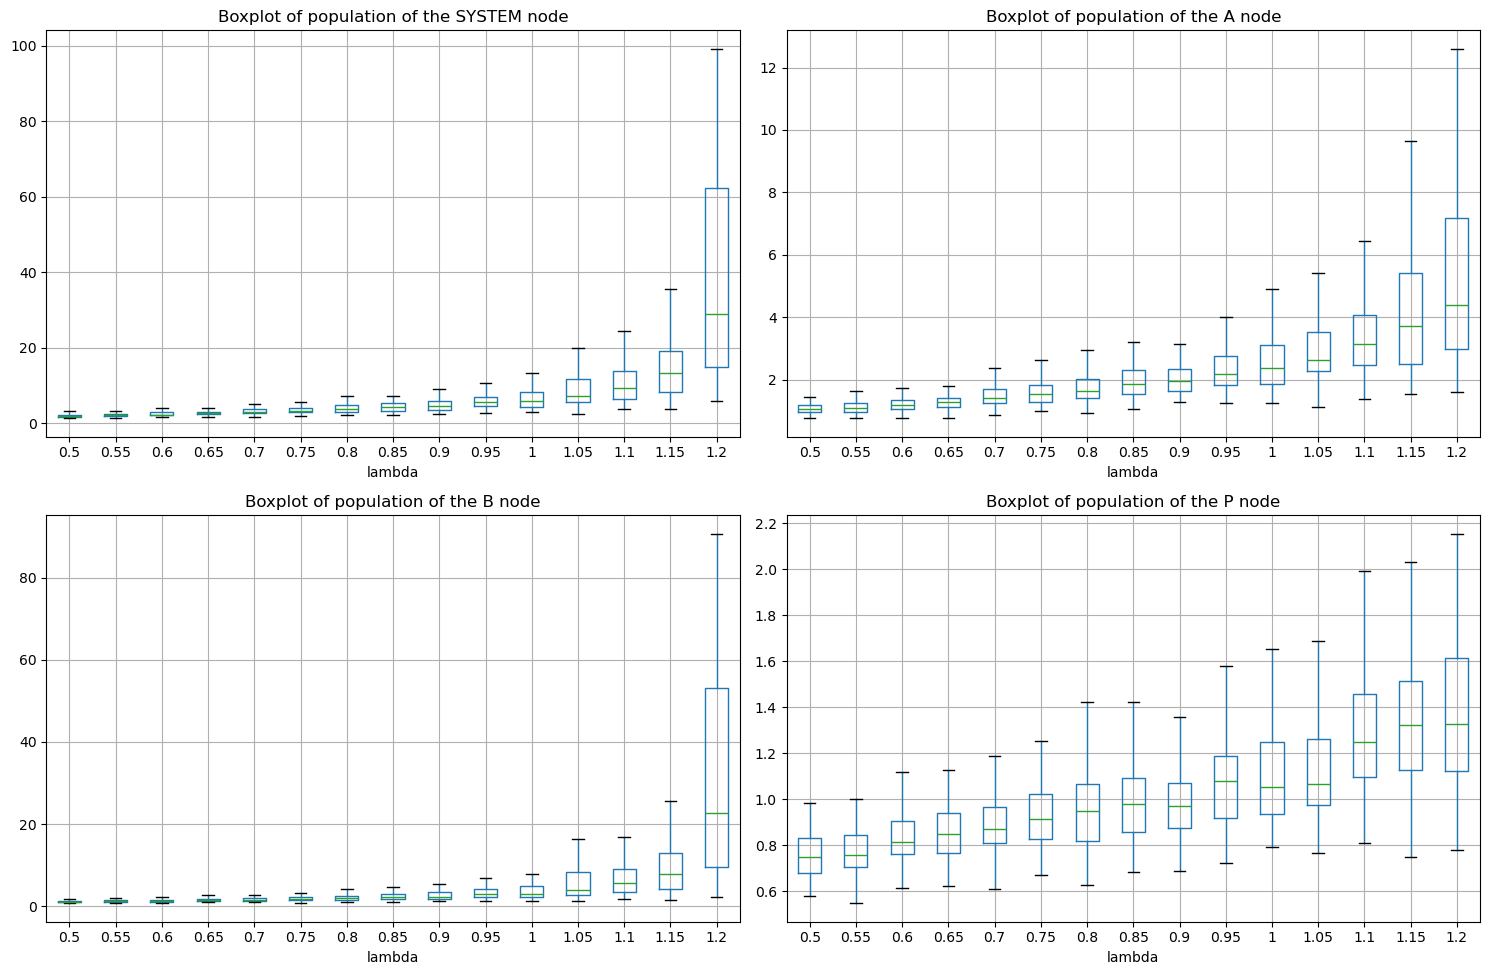
\includegraphics[width=\textwidth]{figs//results/obj1/obj1-box-population.png}
    \caption{Distribuzione della popolazione media dei risultati sperimentali dell'obbiettivo 1.}
    \label{fig:obj1_boxplot_population}
\end{figure*}
Comportamento analogo segue il tempo medio di risposta in \autoref{fig:obj1_boxplot_response_time}, il server P presenta come valore medio massimo 0.78$s$ in corrispondenza del tasso di arrivo massimo, mentre il server A arriva a 1.47$s$. Il server B è in un range più ampio con picchi, per i tassi di arrivo 1.15$job/s$ e 1.2$job/s$, che arrivano a 9.38$s$ e 25.50$s$.
\begin{figure*}
    \centering
    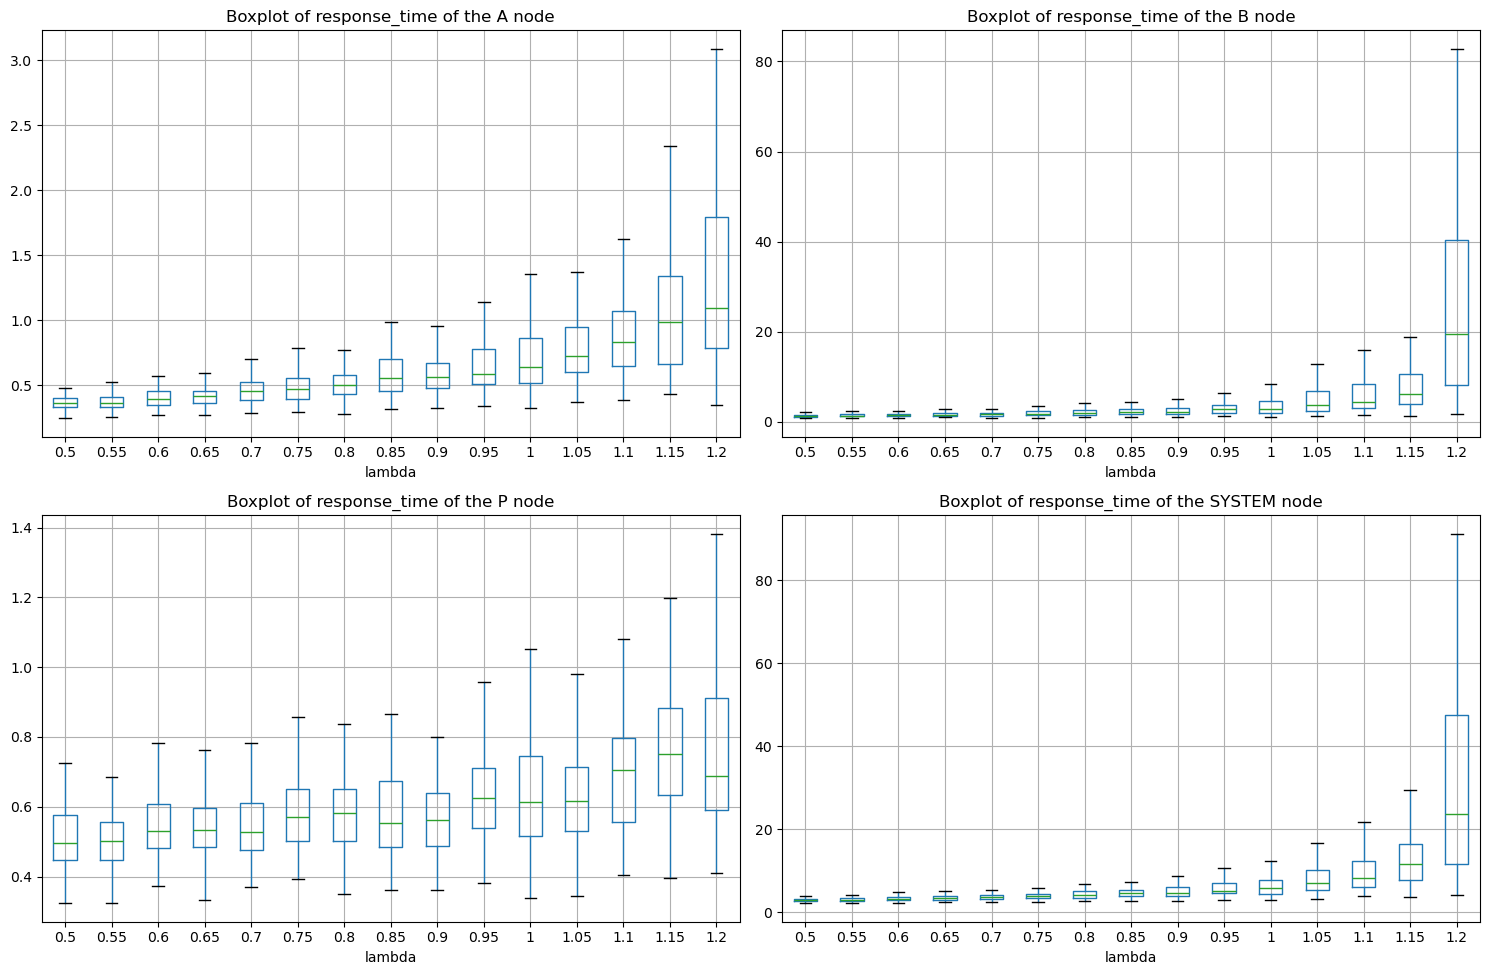
\includegraphics[width=\textwidth]{figs//results/obj1/obj1-box-response-time.png}
    \caption{Distribuzione dei tempi di risposta medi dei risultati sperimentali dell'obbiettivo 1.}
    \label{fig:obj1_boxplot_response_time}
\end{figure*}
Infine per il throughput in \autoref{fig:obj1_boxplot_throughput} tutti e tre i server hanno un andamento costantemente crescente, indice che comunque riescono a servire i job in arrivo. Il server A ha il throughput più alto, mentre B e P hanno un andamento molto simile come si può vedere anche dal grafico in \autoref{fig:obj1_throughput_comparison}

\begin{figure}[H]
    \centering
    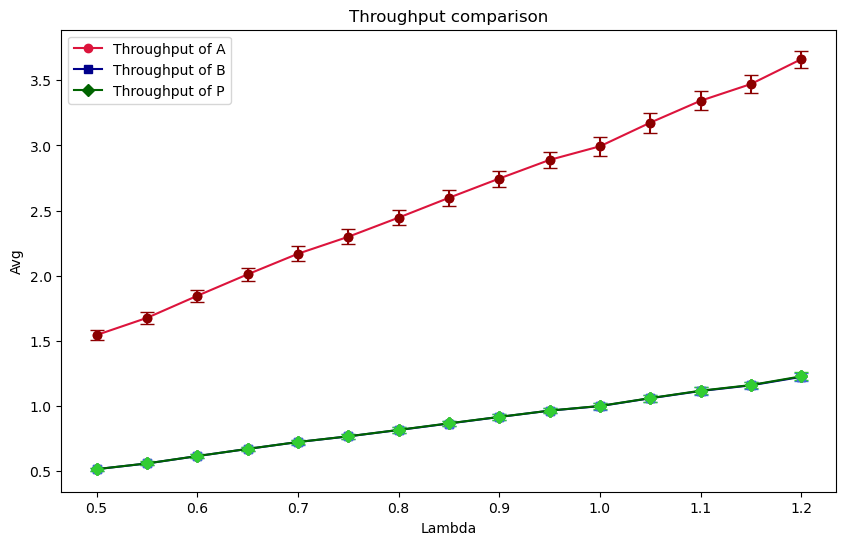
\includegraphics[width=\columnwidth]{figs/results/obj1/obj1-throughput-comparison.png}
    \caption{Confronto throughput per i server A, B e P per l'obiettivo 1}
    \label{fig:obj1_throughput_comparison}
\end{figure}

\begin{figure*}
    \centering
    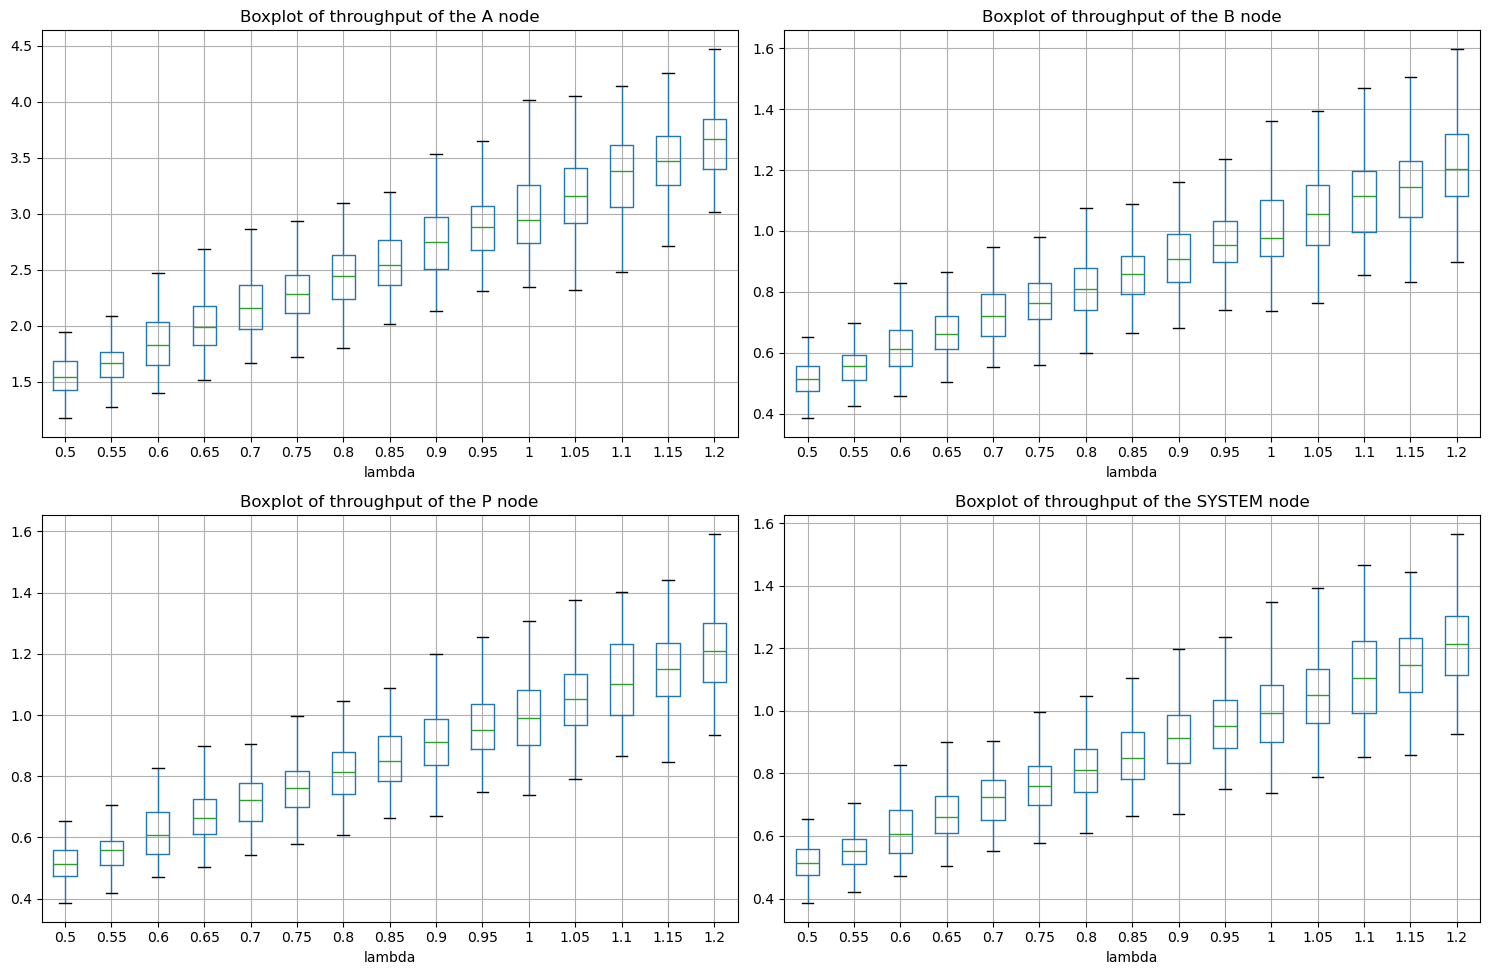
\includegraphics[width=\textwidth]{figs//results/obj1/obj1-box-throughput.png}
    \caption{Distribuzione del throughput medio dei risultati sperimentali dell'obbiettivo 1.}
    \label{fig:obj1_boxplot_throughput}
\end{figure*}


\subsubsection{Verifica con il modello analitico}
Per il tasso di servizio del server A nel modello analitico abbiamo utilizzato i seguenti parametri:
$\displaystyle {\mu}_{A} = 5.833 job/s$.
Mentre i tassi di servizio per i server B e P restano invariati rispetto alla simulazione: $\displaystyle {\mu}_{B} = 1.25job/s$ e $\displaystyle {\mu}_{P} = 2.5job/s$.\\
Per ogni lambda i nodi risultano stabili, riportiamo i valori per tasso di arrivo minimo e massimo:

\begin{table}[!htbp]
    \centering
    \begin{tabular}{cccc}
         $\gamma$ & $\rho_{A}$ & $\rho_{B}$ & $\rho_{P}$\\
         0.5 & 0.257 & 0.4 & 0.2 \\
         1.2	& 0.617 & 0.96 & 0.48 \\
    \end{tabular}
    \label{tab:my_label}
\end{table}

Anche in questo caso riportiamo i valori di ogni indice locale per tasso di arrivo minimo e massimo:

\begin{table}[!htbp]
    \centering
    \begin{tabular}{cccc}
        $\gamma$ & $E[T]_{A}$ & $E[T]_{B}$ & $E[T]_{P}$ \\         
        0.5 & 0.230 & 1.333 & 0.5 \\
        1.2 & 0.447 & 20 & 0.769 \\
    \end{tabular}
    \label{tab:et_values}
\end{table}

\begin{table}[!htbp]
    \centering
    \begin{tabular}{cccc}
        $\gamma$ & $E[N]_{A}$ & $E[N]_{B}$ & $E[N]_{P}$ \\         
        0.5 & 0.346 & 0.666 & 0.25 \\
        1.2 & 1.611 & 24 & 0.923 \\
    \end{tabular}
    \label{tab:en_values}
\end{table}

\begin{table}[!htbp]
    \centering
    \begin{tabular}{cccc}
        $\gamma$ & $X_{A}$ & $X_{B}$ & $X_{P}$ \\         
        0.5 & 1.5 & 0.5 & 0.5 \\
        1.2 & 3.6 & 1.2 & 1.2 \\
    \end{tabular}
    \label{tab:x_values}
\end{table}

Infine segue la tabella per gli indici globali della rete:\\
\begin{table}[H]
    \centering
    \begin{tabular}{cccc}
        $\gamma$ & $E[T]_{S}$ & $E[N]_{S}$ & $X_{S}$ \\         
        0.5 & 2.525 & 1.262 & 0.5 \\
        1.2 & 22.112 & 26.535 & 1.2 \\
    \end{tabular}
    \label{tab:et_en_x_values_last_first}
\end{table}
In \autoref{fig:obj1_line_response_time}, \autoref{fig:obj1_line_population}, \autoref{fig:obj1_line_throughput} è possibile vedere i grafici dell'intervallo di confidenza delle metriche ed il confronto con il modello analitico. Per quanto riguarda la popolazione media i server P e B si discostano molto poco, la differenza è mediamente di 0.5, ad eccezione del server B in corrispondenza del tasso di arrivo massimo dove si vede un discostamento maggiore. Il server A invece presenta un discostamento leggermente superiore, ma comprensibile dato il diverso rate di servizio utilizzato. Possiamo osservare un comportamento analogo per i tempi medi di risposta. Infine il throughput è la metrica che presenta il comportamento migliore aderendo in modo piuttosto preciso.
\begin{figure*}
    \centering
    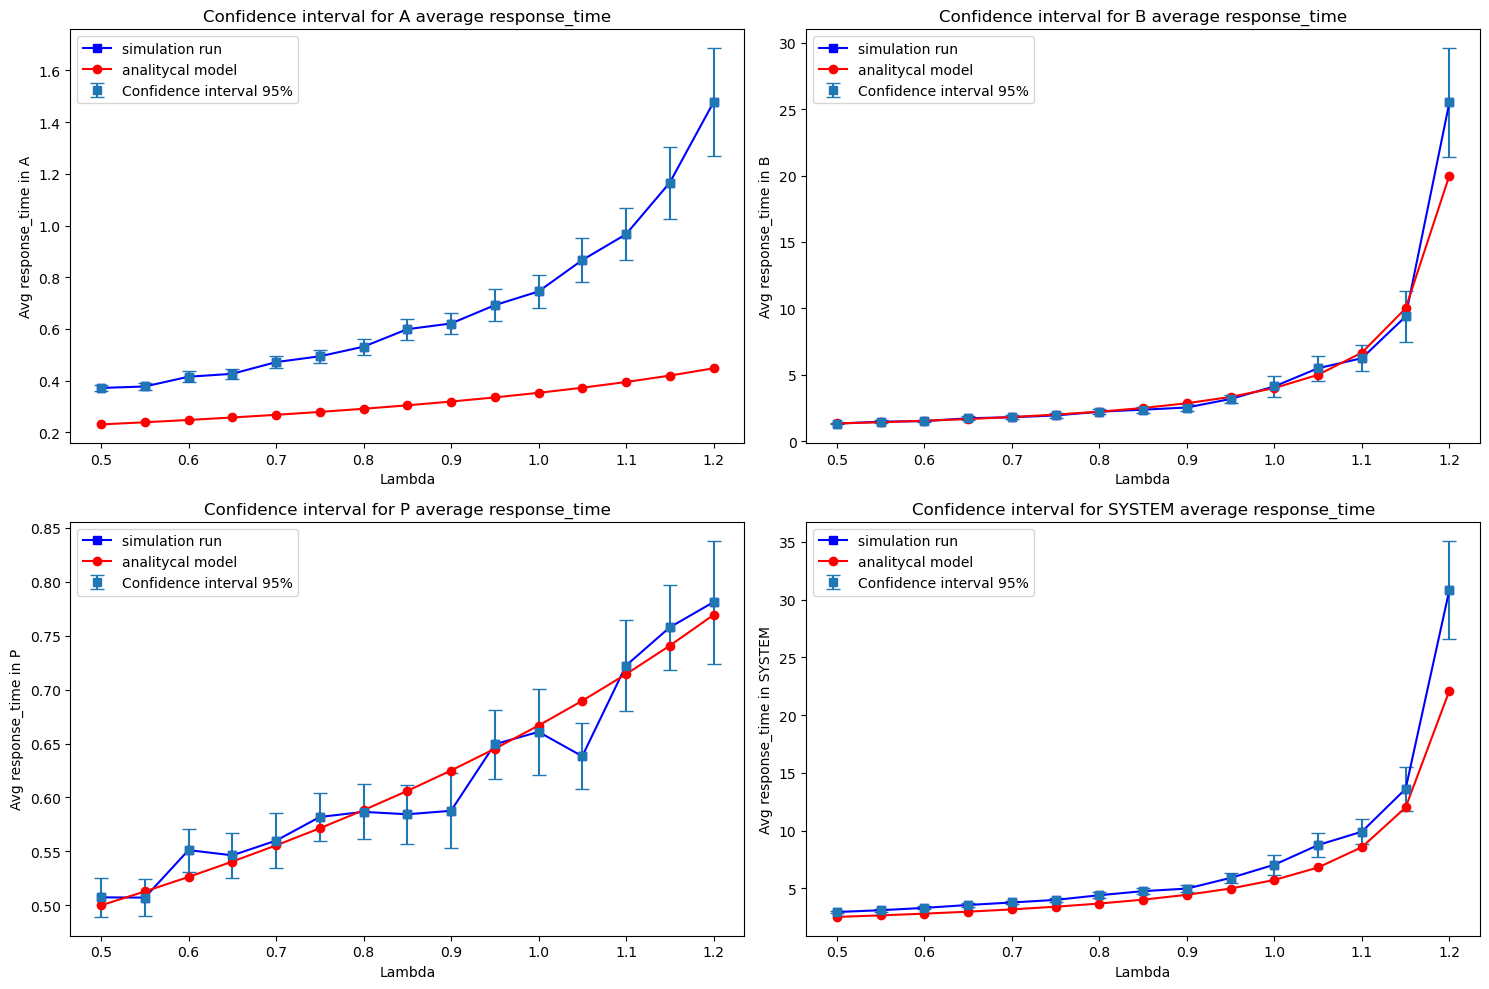
\includegraphics[width=\textwidth]{figs//results/obj1/obj1-line-response-time.png}
    \caption{Intervallo di confidenza del tempo di risposta medio e confronto con modello analitico per l'obiettivo 1}
    \label{fig:obj1_line_response_time}
\end{figure*}
\begin{figure*}
    \centering
    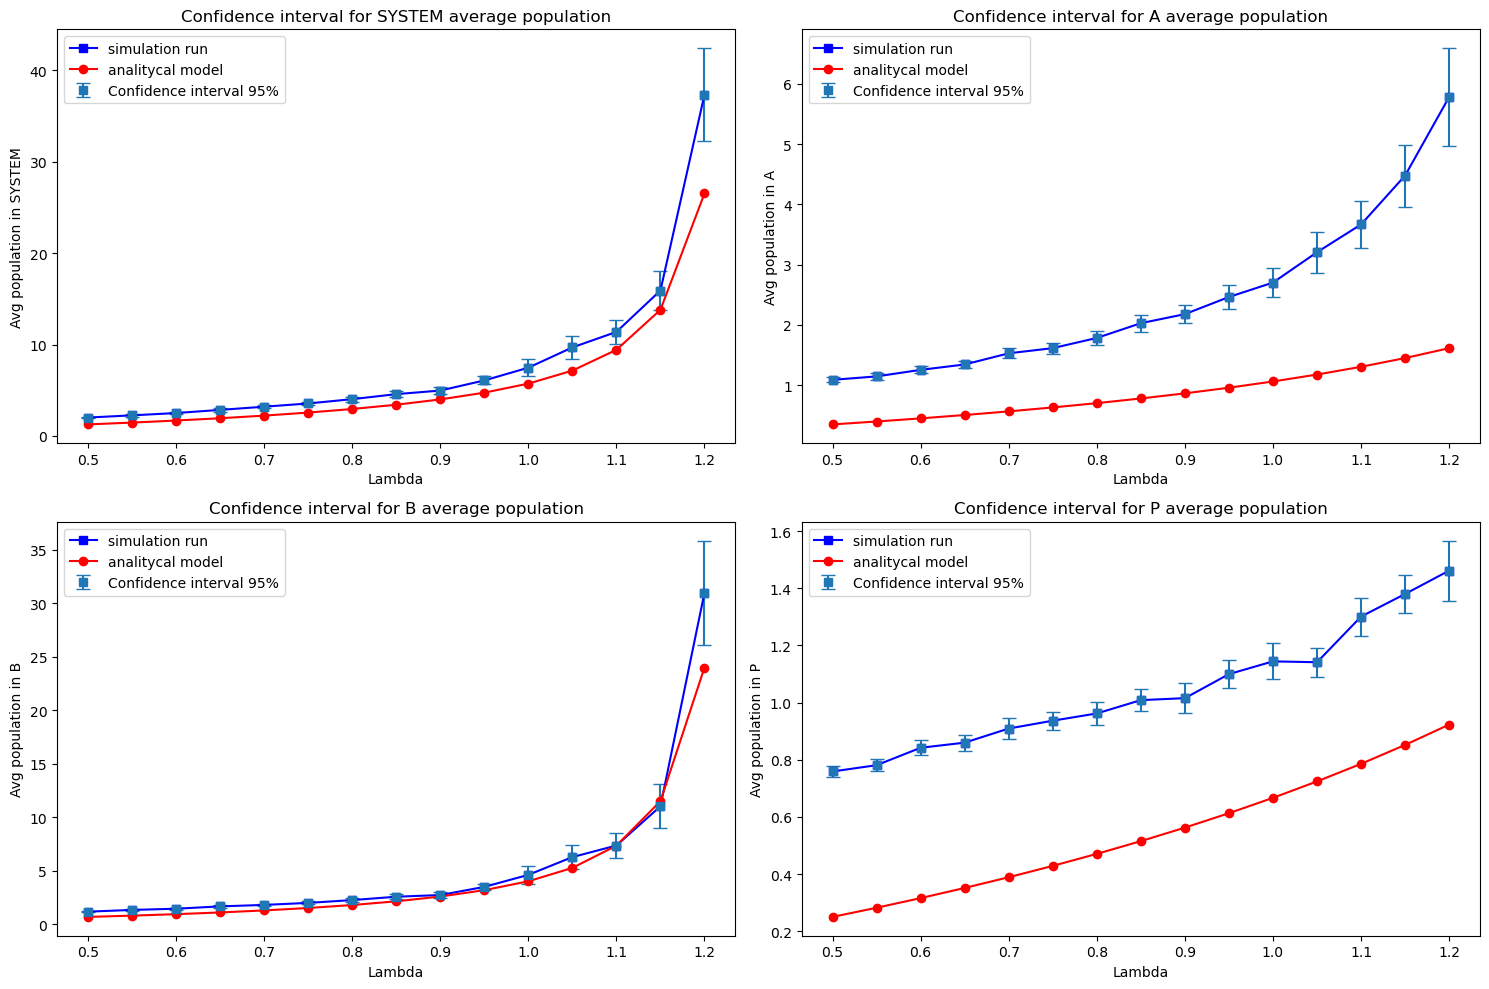
\includegraphics[width=\textwidth]{figs//results/obj1/obj1-line-population.png}
    \caption{Intervallo di confidenza della popolazione media e confronto con modello analitico per l'obiettivo 1}
    \label{fig:obj1_line_population}
\end{figure*}
\begin{figure*}
    \centering
    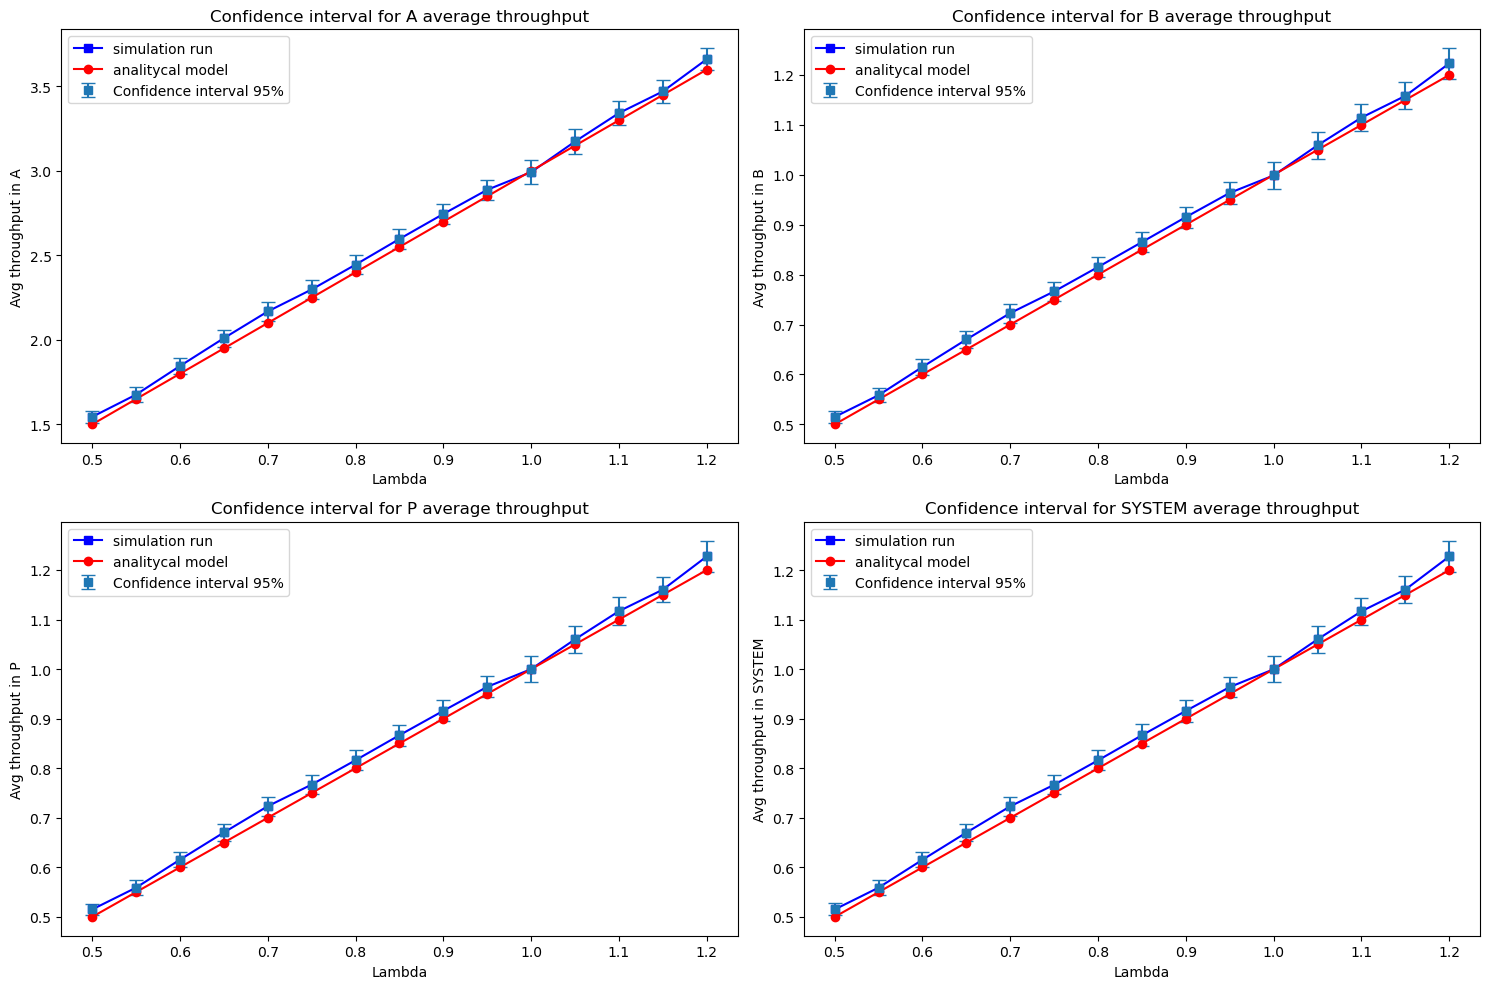
\includegraphics[width=\textwidth]{figs//results/obj1/obj1-line-throughput.png}
    \caption{Intervallo di confidenza del throughput medio e confronto con modello analitico per l'obiettivo 1}
    \label{fig:obj1_line_throughput}
\end{figure*}

Abbiamo effettuato in \autoref{fig:obj1_lineplots_utilization} i grafici anche per l'utilizzazione dei singoli nodi per effettuare i confronti con il modello analitico.\\
Come per il throughput anche in questo caso notiamo una forte aderenza tra i due modelli sempre con il server A più discostato rispetto agli altri due server.
\begin{figure*}
    \centering
    \begin{subfigure}{0.49\linewidth}
        \centering
        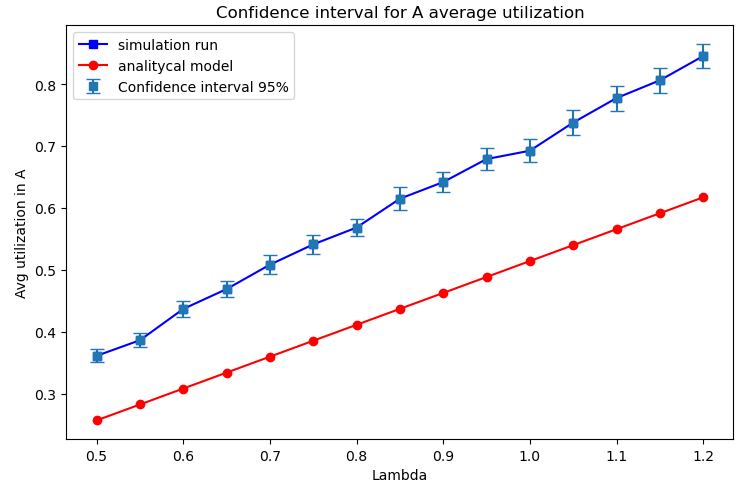
\includegraphics[width=\columnwidth]{figs/results/obj1/obj1-line-utilization-A.png}
        \caption{Server A}
        \label{fig:obj1_line_utilization_A}
    \end{subfigure} 
    \begin{subfigure}{0.49\linewidth}
        \centering
         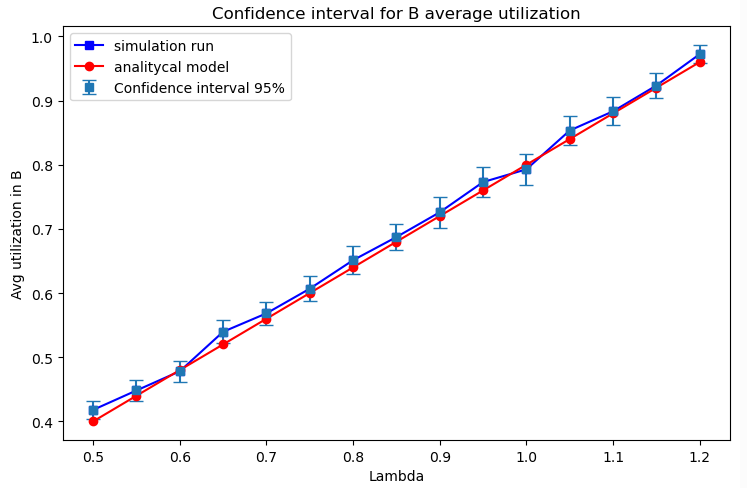
\includegraphics[width=\columnwidth]{figs/results/obj1/obj1-line-utilization-B.png}
        \caption{Server B}
        \label{fig:obj1_line_utilization_B}
    \end{subfigure}
    \begin{subfigure}{0.5\linewidth}
        \centering
        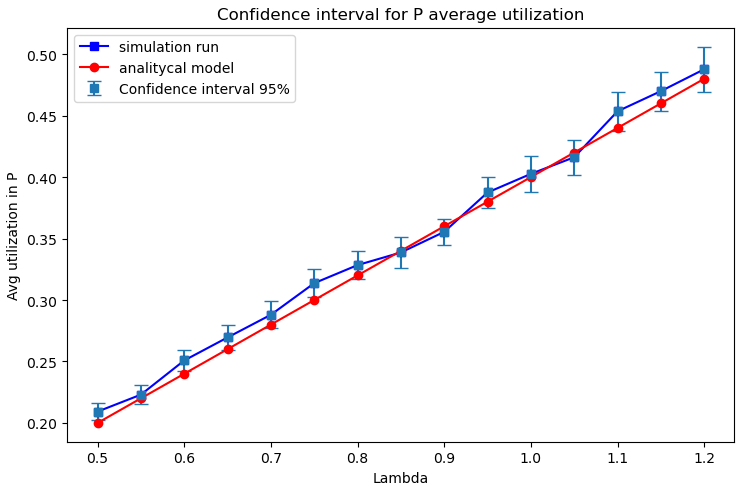
\includegraphics[width=\columnwidth]{figs/results/obj1/obj1-line-utilization-P.png}
        \caption{Server P}
        \label{fig:obj1_line_utilization_P}
    \end{subfigure}
    \caption{Intervallo di confidenza dell'utilizzazione e confronto con modello analitico per l'obiettivo 1.}
    \label{fig:obj1_lineplots_utilization}
\end{figure*}

\subsubsection{Validazione con il caso di studio}
Per la validazione dell'obiettivo 1 si faccia riferimento a \autoref{sec:results_obj2_validation}

\subsubsection{Analisi orizzonte finito}
\label{sec:results-obj1-transient}
Abbiamo infine eseguito una simulazione ad orizzonte finito con 100 run da 64 job ciascuna di cui si possono vedere i risultati in \autoref{fig:obj1_line_population-rep}, \autoref{fig:obj1_line_response_time-rep}, \autoref{fig:obj1_line_throughput-rep} sempre facendo il confronto con i dati ottenuti dal modello analitico, in questo caso notiamo come il modello differisce in maniera più evidente rispetto al caso dell'orizzonte finito, risultato atteso dato che sono statistiche ottenute dal sistema in stato transitorio.
\begin{figure*}
    \centering
    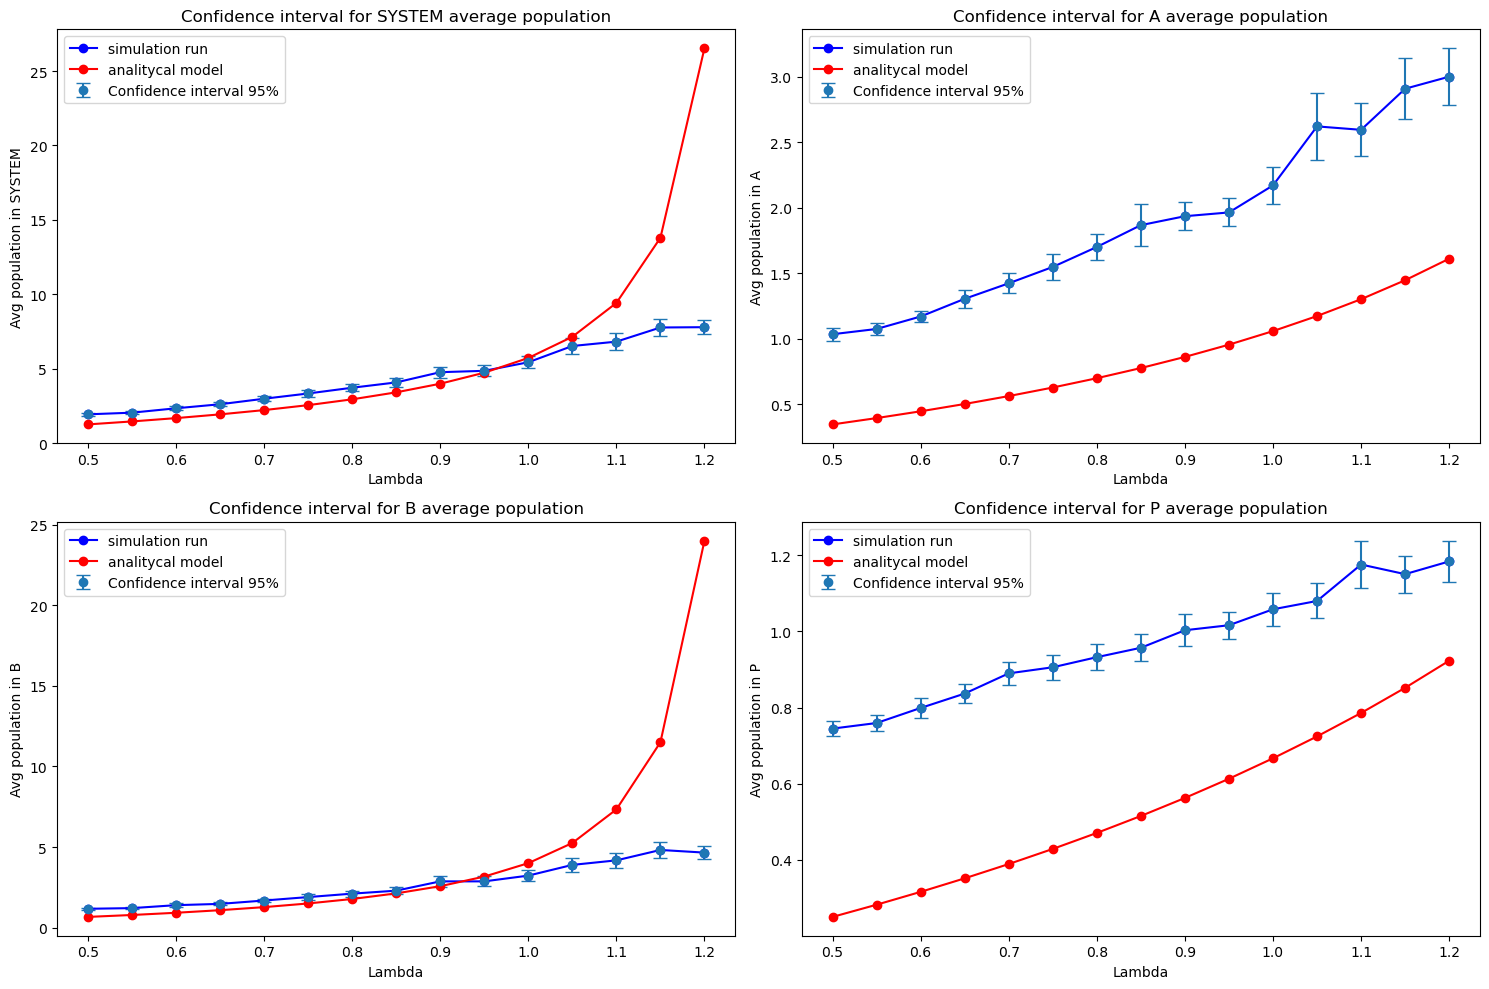
\includegraphics[width=\textwidth]{figs//results/obj1/obj1-line-population-rep.png}
    \caption{Intervallo di confidenza della popolazione media e confronto con modello analitico per l'obiettivo 1 ad orizzonte finito.}
    \label{fig:obj1_line_population-rep}
\end{figure*}
\begin{figure*}
    \centering
    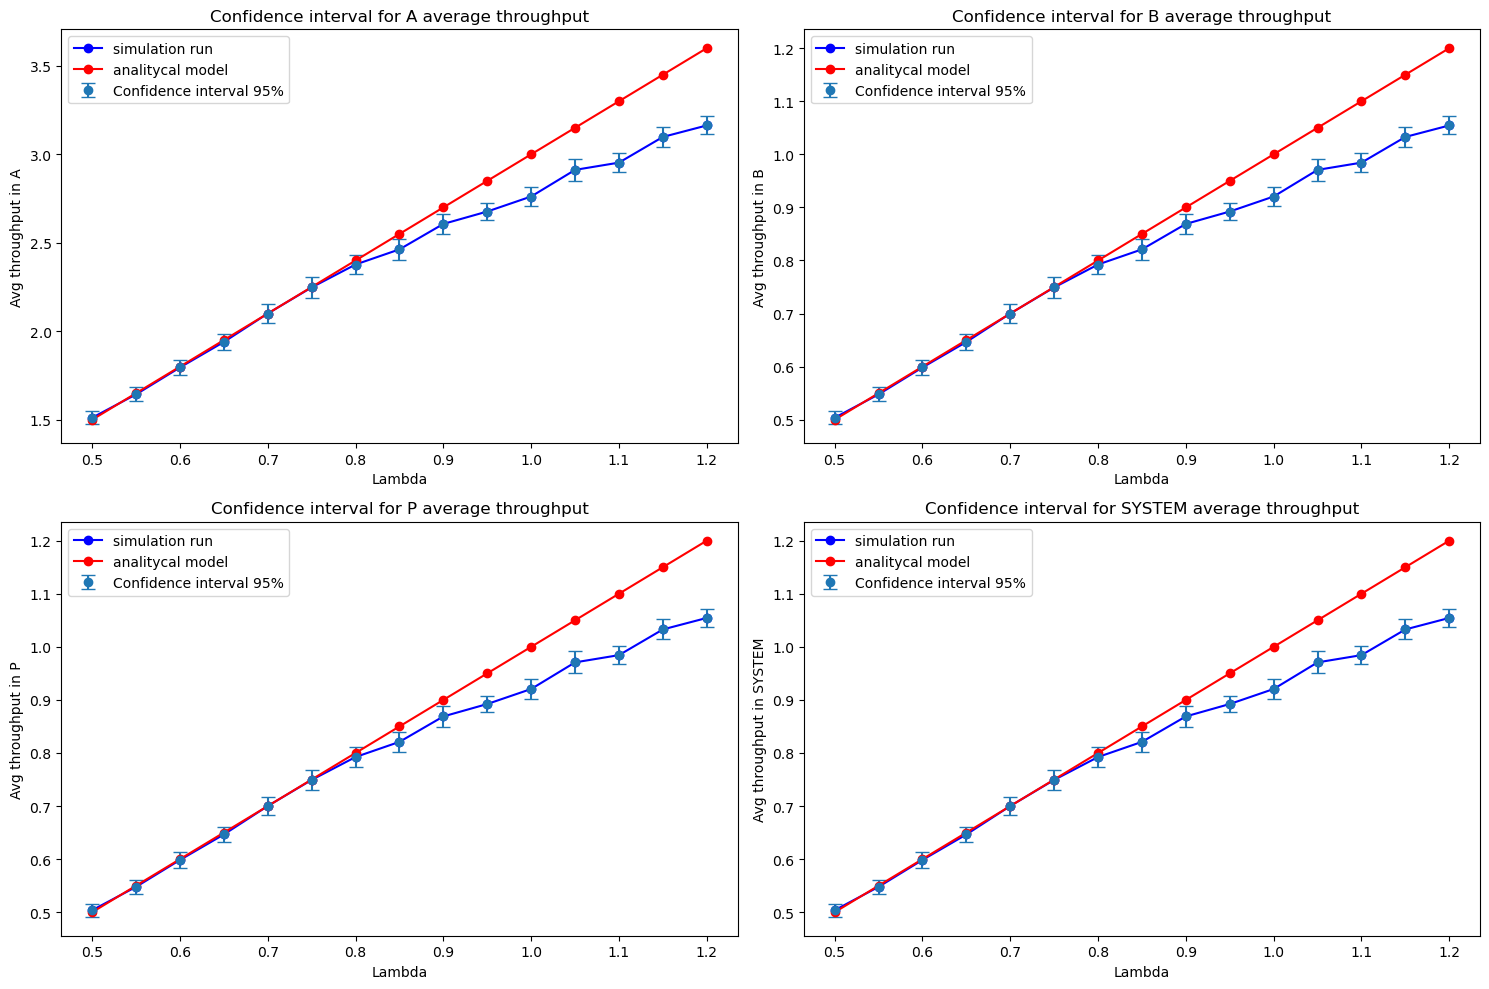
\includegraphics[width=\textwidth]{figs//results/obj1/obj1-line-throughput-rep.png}
    \caption{Intervallo di confidenza del throughput medio e confronto con modello analitico per l'obiettivo 1 ad orizzonte finito.}
    \label{fig:obj1_line_throughput-rep}
\end{figure*}
\begin{figure*}
    \centering
    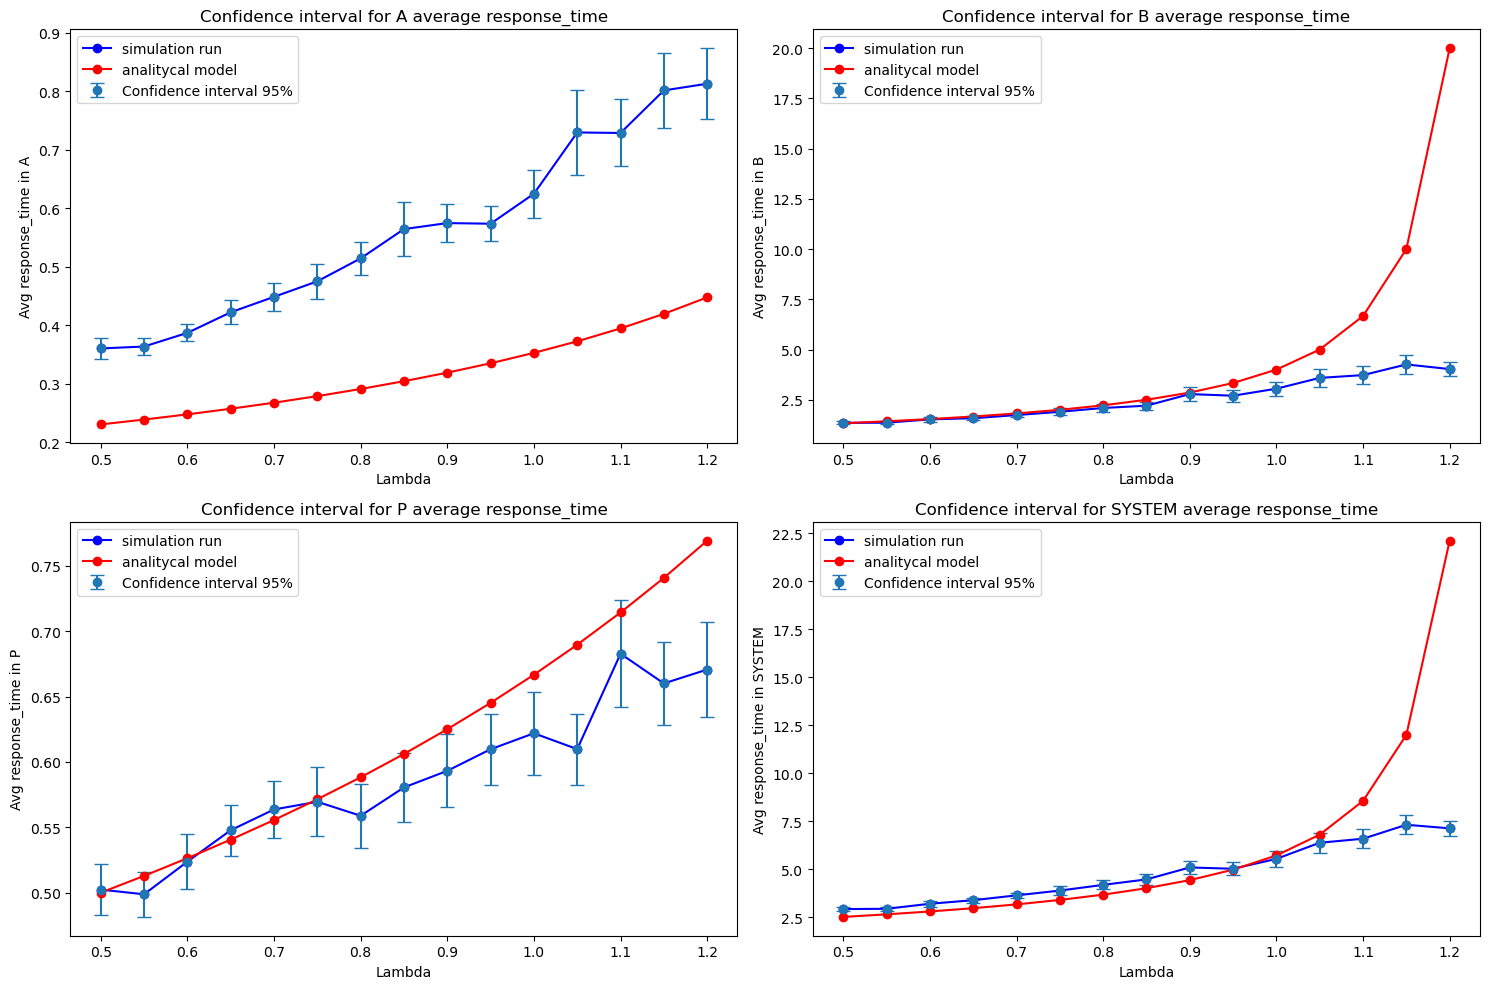
\includegraphics[width=\textwidth]{figs//results/obj1/obj1-line-response-time-rep.png}
    \caption{Intervallo di confidenza del tempo di risposta medio e confronto con modello analitico per l'obiettivo 1 ad orizzonte finito.}
    \label{fig:obj1_line_response_time-rep}
\end{figure*}
